\noindent \textbf{Paraphrase variation concentration in nuisance directions.}
To quantify whether paraphrase-induced variation is concentrated in the discovered nuisance subspace, we measure the fraction of within-group paraphrase variation captured by that subspace. For a semantic group
\[
g=\{x_1,\ldots,x_k\},
\]
let
\[
z_i=\Phi_\ell(x_i)
\]
denote the latent representation at layer $\ell$ for the $i$-th paraphrase, and let the group centroid be
\[
\bar z_g
=
\frac1k
\sum_{i=1}^k z_i.
\]
Define each paraphrase deviation from the centroid as
\[
\delta_i=z_i-\bar z_g.
\]
These deviations characterize within-group paraphrase variation. We then compute the fraction of this variation captured by the nuisance subspace:
\[
R_{\mathrm{nuis}}
=
\frac{
\sum_i
\|P_{T^{\mathrm{nuis}}}\delta_i\|_2^2
}{
\sum_i
\|\delta_i\|_2^2
}.
\]
The numerator measures how much paraphrase variation lies inside the nuisance subspace, while the denominator measures total paraphrase variation. Thus,
\[
R_{\mathrm{nuis}}\approx 1
\]
indicates that paraphrastic variation is largely confined to nuisance directions, supporting the tangent-space hypothesis.

As a simple toy illustration, suppose paraphrase deviations are
\[
\delta_1=
\begin{bmatrix}
0.2\\
0.2\\
0
\end{bmatrix},
\qquad
\delta_2=
\begin{bmatrix}
-0.1\\
-0.1\\
0
\end{bmatrix},
\]
and the nuisance direction is
\[
v_1=
\frac1{\sqrt2}
\begin{bmatrix}
1\\
1\\
0
\end{bmatrix}.
\]
Since these deviations lie nearly entirely along $v_1$, their projections preserve almost all of their energy, yielding
\[
R_{\mathrm{nuis}}\approx 1.
\]
Combined with a small projection-energy measure
\[
E_{\mathrm{nuisance}},
\]
which indicates semantic displacement lies largely outside nuisance directions, these two quantities provide complementary validation of the geometric hypothesis:
\[
R_{\mathrm{nuis}}\uparrow
\quad\text{and}\quad
E_{\mathrm{nuisance}}\downarrow.
\]
The former shows paraphrases move primarily in nuisance directions, while the latter shows semantic separation occurs largely outside them.
% \textbf{7. Tangent-Direction Decomposition Experiment}
% For each semantic group (prompt + paraphrases), compute the local variation subspace.
% If the hypothesis is correct:
% paraphrase differences lie in low-rank nuisance directions

% Q: Do paraphrases actually move along a low-dimensional nuisance subspace?

% \paragraph{Procedure.}
% To empirically examine the local geometric hypothesis introduced in Section 3, we analyze whether paraphrastic variation primarily occurs along low-dimensional nuisance directions while semantic differences lie in orthogonal directions. The experiment estimates a local tangent subspace induced by paraphrases and evaluates how semantic separation relates to that subspace.

% Let $\Phi_\ell(x)\in\mathbb{R}^d$ denote the pooled latent representation of input $x$ at layer $\ell$. For each semantic group $g$ consisting of $k$ paraphrases $\{x_1,\dots,x_k\}$, we collect their representations
% \[
% Z_g = [z_1, z_2, \dots, z_k], \qquad z_i = \Phi_\ell(x_i).
% \]

% \paragraph{Step 1: Local representation centering.}
% We first compute the group centroid
% \[
% \bar z_g = \frac{1}{k}\sum_{i=1}^{k} z_i ,
% \]
% and construct the centered representation matrix
% \[
% \tilde Z_g = [z_1-\bar z_g,\; z_2-\bar z_g,\; \dots,\; z_k-\bar z_g].
% \]

% \paragraph{Step 2: Estimating nuisance tangent directions.}
% We perform principal component analysis on $\tilde Z_g$ and obtain the principal directions $\{v_1, v_2, \dots\}$.  
% The leading components span a low-dimensional subspace that approximates the local nuisance tangent space induced by paraphrasing,
% \[
% T^{\text{nuisance}}_g = \mathrm{span}(v_1,\dots,v_r),
% \]
% where $r$ is a small integer (typically $r=1$ or $2$).

% \paragraph{Step 3: Semantic difference vectors.}
% For two semantic groups $g$ and $h$, we compute their centroid difference
% \[
% \Delta_{gh} = \bar z_g - \bar z_h ,
% \]
% which represents the semantic displacement between the two meaning clusters in latent space.

% \paragraph{Step 4: Projection energy.}
% To measure whether semantic variation aligns with nuisance directions, we compute the fraction of semantic displacement energy that lies within the nuisance subspace,
% \[
% E_{\text{nuisance}} =
% \frac{\|P_{T^{\text{nuisance}}_g}\Delta_{gh}\|^2}
% {\|\Delta_{gh}\|^2},
% \]
% where $P_{T^{\text{nuisance}}_g}$ denotes the orthogonal projection operator onto the estimated nuisance subspace.

% \paragraph{Interpretation.}
% If the local geometric hypothesis holds, paraphrase variations should lie predominantly within the nuisance tangent subspace while semantic differences should occur largely outside it. Consequently, invariant layers are expected to exhibit small values of $E_{\text{nuisance}}$, indicating that semantic separation occurs primarily along directions orthogonal to paraphrase-induced variation.




\noindent \textbf{7. Tangent-Direction Validation of Discovered Invariant Geometry.}
This experiment is designed as validation of the geometric decomposition in Section 3.2 rather than as a second discovery procedure. Its purpose is to test whether paraphrastic variation indeed concentrates in the nuisance subspace identified by contrastive sensitivity decomposition, and whether semantic displacement lies largely outside that subspace.

Let
\[
U_\ell^{\mathrm{nuis}}
=
[v_{k+1},\ldots,v_d]
\]
denote the nuisance subspace basis at layer $\ell$, formed by the generalized eigenvectors associated with the smaller generalized eigenvalues in
\[
S_{sc}^{\ell} v = \lambda S_{sp}^{\ell} v.
\]
Unlike a separate PCA fitted per semantic group, this experiment directly uses the nuisance directions already discovered in Section 3.2, making it a validation of the learned geometric structure rather than an alternative estimator.

For each semantic group
\[
g=\{x_1,\ldots,x_k\},
\]
let
\[
z_i=\Phi_\ell(x_i)
\]
be their latent representations, and define the group centroid
\[
\bar z_g
=
\frac1k
\sum_{i=1}^k z_i.
\]

For another semantic group \(h\), define the semantic displacement
\[
\Delta_{gh}
=
\bar z_g-\bar z_h.
\]

We form the orthogonal projector onto the nuisance subspace:
\[
P_{T^{\mathrm{nuis}}}
=
U_\ell^{\mathrm{nuis}}
U_\ell^{\mathrm{nuis}\top}.
\]

We then measure how much semantic displacement lies inside the nuisance subspace via projection energy:
\[
E_{\mathrm{nuisance}}
=
\frac{
\|P_{T^{\mathrm{nuis}}}\Delta_{gh}\|_2^2
}{
\|\Delta_{gh}\|_2^2
}.
\]

Small values of
\[
E_{\mathrm{nuisance}}
\]
indicate that semantic separation occurs largely outside the nuisance subspace, consistent with the geometric hypothesis that paraphrase-induced variation and semantic variation occupy distinct directions.

\noindent\textbf{Toy illustration.}
Consider the nuisance direction
\[
v_1=
\frac1{\sqrt2}
\begin{bmatrix}
1\\
1\\
0
\end{bmatrix}
\]
so
\[
P_{T^{\mathrm{nuis}}}
=
v_1v_1^\top.
\]
Suppose the semantic displacement between two concept groups is
\[
\Delta_{gh}
=
\begin{bmatrix}
2\\
-2\\
3
\end{bmatrix}.
\]
Its projection onto the nuisance subspace is
\[
P_{T^{\mathrm{nuis}}}\Delta_{gh}
=
v_1v_1^\top \Delta_{gh}.
\]
Since
\[
v_1^\top \Delta_{gh}
=
\frac{2-2}{\sqrt2}
=0,
\]
we obtain
\[
P_{T^{\mathrm{nuis}}}\Delta_{gh}=0
\]
and therefore
\[
E_{\mathrm{nuisance}}=0.
\]
This means semantic displacement lies entirely outside the nuisance directions, exactly matching the geometric hypothesis.

Unlike Section 3.2, which discovers invariant and nuisance subspaces, this experiment tests whether those discovered directions actually exhibit the predicted tangent-space behavior in practice. 
















We construct a controlled evaluation environment designed to isolate semantic invariance from surface-form variation across a diverse set of transformer-based language models.

\paragraph{Dataset Construction.}

\begin{table}[h]
\centering
\vspace{4pt}
\begin{tabular}{lcc}
\toprule
\textbf{Thematic Group} & \textbf{SP Variants} & \textbf{SC Variants} \\
\midrule
Cats           & 10 & 10 \\
France         & 10 & 10 \\
Python         & 10 & 10 \\
Photosynthesis & 10 & 10 \\
Democracy      & 10 & 10 \\
Einstein       & 10 & 10 \\
Climate Change & 10 & 10 \\
Calculus       & 10 & 10 \\
Meditation     & 10 & 10 \\
Bread          & 10 & 10 \\
\midrule
\textbf{Total} & \textbf{100} & \textbf{100} \\
\bottomrule
\end{tabular}
\caption{Dataset composition across thematic groups. Each group contributes one anchor query, 10 semantically preserving (SP) paraphrases, and 10 semantically changing (SC) variants, yielding 210 sentences in total (10 anchors + 100 SP + 100 SC).}
\label{tab:dataset_category}
\vspace{-2.0em}
\end{table}

Our dataset consists of 210 prompts organized into 10 thematic groups spanning diverse semantic domains, as summarized in Table~\ref{tab:dataset_category}. The groups cover topics including Cats, France, Python, Photosynthesis, Democracy, Einstein, Climate Change, Calculus, Meditation, and Bread, each representing a distinct conceptual domain. For each group, one anchor query is selected from one of five query types (Factual, Procedural, Descriptive, Opinion, or Causal), chosen to maximize diversity in linguistic form and semantic content across groups. For each anchor query, we construct two families of controlled perturbations:

\begin{itemize}
    \item \textbf{Semantically Preserving (SP) variants:} Ten paraphrases per anchor that preserve propositional content while varying surface form through lexical substitution, syntactic restructuring, and perspectival rephrasing, ensuring no two SP variants share the same syntactic template.
    \item \textbf{Semantically Changing (SC) variants:} Ten modified sentences per anchor constructed through surgical substitution of a single semantic slot — subject, predicate, or object — while preserving syntactic structure, register, and sentence length. This controlled construction ensures that observed differences in representation space are attributable to semantic content rather than confounded by surface-level variation.
\end{itemize}

\xz{1: do we talk about easy and hard SC? 2: show one group example?}

This yields 21 sentences per group (1 anchor + 10 SP + 10 SC) and 210 sentences in total. Each group defines one \textit{concept unit}, so all within-group comparisons are anchored to the same original query.

\paragraph{Within--Across Experimental Design.}
The dataset operationalizes representational invariance directly: a representation is invariant if it changes less under meaning-preserving transformations (SP perturbations) than under meaning-changing transformations (SC perturbations). All analyses compare these two conditions at each layer - within-concept stability under SP versus across-concept sensitivity under SC - and the degree to which the two are separated constitutes the invariance signal. Because all variants share a common anchor and construction procedure, any observed separation cannot be attributed to differences in sentence length, syntactic complexity, or domain.

\paragraph{Models Analyzed.}

\begin{table}[h]
\centering
\begin{tabular}{llc}
\toprule
\textbf{Model} & \textbf{Family} & \textbf{Parameters} \\
\midrule
Mistral-7B-Instruct-v0.3      & Mistral    & 7B \\
Meta-Llama-3-8B-Instruct      & Llama      & 8B \\
Gemma-7B-IT                   & Gemma      & 7B \\
Qwen2.5-7B-Instruct           & Qwen       & 7B \\
GLM-4-9B-Chat                 & GLM        & 9B \\
DeepSeek-MoE-16B-Chat         & DeepSeek   & 16B \\
InternLM2-Chat-7B             & InternLM   & 7B \\
Phi-4-Mini-Instruct           & Phi        & 4B \\
Falcon3-7B-Instruct           & Falcon     & 7B \\
\bottomrule
\end{tabular}
\caption{Transformer-based decoder-only language models evaluated for representational invariance. Models span diverse architectural families, training objectives, and parameter scales.}
\label{tab:models}
\vspace{-2.0em}
\end{table}

We evaluate nine transformer-based decoder-only language models listed in Table~\ref{tab:models}, spanning diverse architectural families, training procedures, and parameter scales ranging from 4B to 9B. The suite includes both instruction-tuned and distilled variants, allowing us to assess whether invariance structure is preserved across different training objectives. All models are evaluated in inference mode with no fine-tuning or prompt engineering applied during representation extraction.




\subsection{Within group Ablation Study: Causal Validation via Representation Intervention}

To validate that the invariant subspace identified through the generalized eigenvalue analysis causally encodes semantic content, we conduct a representation intervention ablation. Rather than observing correlational properties of the representations, this experiment directly intervenes on the hidden states at each layer and measures the effect on the model's output distribution. If the invariant subspace genuinely captures semantic meaning, then replacing it with semantically different content should produce a measurable shift in the output, while replacing it with semantically equivalent content should not.

\paragraph{Decomposition and Projection.}
For each transformer layer $l$, the invariant subspace is defined by the top-$k$ eigenvectors $U_{\mathrm{inv}} \in \mathbb{R}^{d \times k}$ obtained from the generalized eigenvalue problem described in Section~3. Given a hidden state vector $h \in \mathbb{R}^d$ at the final token position of a sentence, we decompose it into two orthogonal components using the general projection formula:

% \begin{align}
%     h_{\mathrm{inv}}  &= U_{\mathrm{inv}} (U_{\mathrm{inv}}^\top U_{\mathrm{inv}})^{-1} U_{\mathrm{inv}}^\top \, h \\
%     h_{\mathrm{nuis}} &= h - h_{\mathrm{inv}}
% \end{align}

\begin{align}
    h_{\mathrm{inv}}  &= P_{\mathrm{inv}} \, h, \quad P_{\mathrm{inv}} = U_{\mathrm{inv}} U_{\mathrm{inv}}^\top \\
    h_{\mathrm{nuis}} &= h - h_{\mathrm{inv}}
\end{align}

The invariant component $h_{\mathrm{inv}}$ lies in the $k$-dimensional subspace spanned by the top-$k$ eigenvectors and represents the directions most sensitive to semantic change relative to paraphrase variation. The nuisance component $h_{\mathrm{nuis}}$ captures the remaining $(d - k)$-dimensional complement, encoding surface-form, syntactic, and other non-semantic variation. By construction, $h = h_{\mathrm{inv}} + h_{\mathrm{nuis}}$ exactly.

\paragraph{Intervention Procedure.}
For each concept group, we select an anchor sentence and pair it with a donor sentence drawn from either the SC or SP family. The intervention replaces the invariant component of the anchor's hidden state at layer $l$ with the invariant component of the donor's hidden state, while leaving the nuisance component unchanged:

\begin{equation}
    h_{\mathrm{intervened}} = h_{\mathrm{anchor}} + \alpha \left( h_{\mathrm{donor,inv}} - h_{\mathrm{anchor,inv}} \right)
\end{equation}

where $\alpha = 1.0$ corresponds to a full hard swap. The modified vector is substituted at the final token position of the anchor sentence's hidden state at layer $l$, and the model's remaining layers $l{+}1$ through $L$ process the modified representation, producing output logits $\hat{p}_{\mathrm{intervened}}$. A corresponding unmodified forward pass produces baseline logits $\hat{p}_{\mathrm{base}}$. A corresponding unmodified forward pass produces baseline logits $\hat{p}_{\mathrm{base}}$. The output shift is measured as the KL divergence between the two next-token distributions:


\begin{equation}
    \mathrm{KL}(l) = D_{\mathrm{KL}}\!\left(\hat{p}_{\mathrm{base}} \,\|\, \hat{p}_{\mathrm{intervened}}\right)
\end{equation}

This is computed at the final token position, which in causal language models aggregates contextual information from the full input sequence and drives next-token prediction. We average $\mathrm{KL}(l)$ over all SC and SP donors respectively to obtain per-layer mean values.

\paragraph{Experimental Conditions.}
We evaluate two swap conditions for the invariant component:

\begin{itemize}
    \item \textbf{Invariant swap with SC donor:} the anchor's invariant component is replaced with that of a semantically different sentence. If the subspace captures semantic content, this should produce a large KL divergence, as the model's downstream prediction is driven by semantically incongruent information.
    \item \textbf{Invariant swap with SP donor:} the anchor's invariant component is replaced with that of a paraphrase. Since both sentences share the same propositional content, the intervened representation should remain semantically consistent with the anchor, producing a small KL divergence.
\end{itemize}

The gap between these two conditions at each layer — $\mathrm{KL}_{\mathrm{SC}} > \mathrm{KL}_{\mathrm{SP}}$ — constitutes the causal evidence that the invariant subspace encodes semantic content rather than surface-form features. Nuisance swap conditions (replacing $h_{\mathrm{nuis}}$ instead of $h_{\mathrm{inv}}$) are reported in Appendix~\ref{app:nuisance_swap} for completeness.

\vspace{-0.8em}
\paragraph{Results.}
We set $k = 32$ invariant directions for all experiments reported here. Figure~\ref{fig:patching_kl} shows the per-layer KL divergence for invariant component swaps across all nine models in a $3 \times 3$ grid, for the best-performing concept group selected for demonstration purposes. Results for all remaining groups are included in Appendix~\ref{app:all_groups}. Each subplot shows two curves: the orange curve corresponds to swaps where the invariant component is replaced with that of a semantically different SC donor, and the blue dotted curve corresponds to swaps where it is replaced with that of a paraphrase SP donor. Across all nine models, the SC curve rises consistently with layer depth while the SP curve remains relatively stable and near zero, producing a clear and growing separation between the two conditions across middle and later layers. This indicates that substituting the invariant component with semantically different content produces a measurable and increasing output shift, whereas substituting it with a paraphrase does not meaningfully perturb the model's predictions. The separation is most pronounced in mid to late layers across the majority of architectures. For the most part, early layers show minimal divergence between the two curves, consistent with the interpretation that lower layers encode primarily syntactic and surface-form features before semantic abstraction consolidates at mid-to-late depth.

The result validates two claims simultaneously. First, the invariant subspace is causally relevant: modifying it changes the model's behavior in a way that is measurable at the output. Second, the causal effect is semantically selective: the output shift is larger when the donor carries different propositional content (SC) than when it carries equivalent content (SP), demonstrating that the subspace specifically encodes semantic meaning rather than arbitrary representational dimensions. The results of the nuisance swap are reported in Appendix~\ref{app:nuisance_swap}.



\begin{figure}[h]
    \centering
    \includegraphics[width=0.8\linewidth]{figures/heatmap_einstein.png}
    \caption{Per-layer eigenvalue heatmap for $k = 32$ invariant directions. Each row corresponds to one eigenvector rank (rank 0 at top) and each column to a transformer layer, with color encoding the $\log_{10}(\lambda)$ value. Brighter cells indicate directions with stronger semantic invariance at that layer. The heatmap complements Figure~\ref{fig:eigenvalue_profiles} by making the joint distribution of rank and layer visible simultaneously, highlighting which layer-rank combinations concentrate the most invariant signal.}
    \label{fig:eigenvalue_heatmap}
\end{figure}

\subsection{Localization of Invariant Feature Zones}
\label{sec: localize}
A central question in our analysis is where in the network semantic invariance concentrates — that is, which layers encode the strongest separation between meaning-preserving and meaning-changing perturbations. To investigate this, we compute the generalized eigenvalue spectrum at every transformer layer and examine how the top eigenvalues are distributed across layers and ranks.



\ad{Heatmap and lambda profiles. Keep one?}

Figure~\ref{fig:eigenvalue_profiles} shows the per-layer eigenvalue profiles for $k = 32$ directions, plotted on a log scale, for one representative model and concept group shown here for demonstration purposes. Each line corresponds to one eigenvector rank, with rank 0 representing the direction of maximal invariance at that layer. Two consistent trends emerge across all models. First, eigenvalues increase steadily with layer depth, indicating that the invariant signal strengthens as representations pass through deeper layers of the network. Second, higher-ranked directions consistently exhibit larger eigenvalues within each layer, confirming that the generalized eigenvalue problem produces a meaningful and ordered decomposition in which some directions are genuinely more semantically selective than others rather than assigning arbitrary or uniform importance across ranks.

The selection of $k$ is a foundational choice in our framework, as it directly determines the dimensionality of the invariant subspace used in all downstream analyses. The top-$k$ eigenvectors span the subspace into which hidden states are projected to isolate semantic content from surface-form variation, and all subsequent experiments — including the causal intervention study and the attribution analysis — operate exclusively within this subspace. A larger $k$ captures a broader portion of the invariant signal at the cost of including directions with progressively weaker semantic selectivity, while a smaller $k$ is more conservative but risks discarding meaningful invariant structure. We empirically select $k = 32$ for all experiments reported in this work. While a smaller $k$ captures the most prominent invariant directions, we find only minor differences in downstream evaluation results when reducing $k$, indicating a degree of insensitivity to this hyperparameter choice within the range tested. For completeness, Appendix~\ref{app:k_comparison} includes comparison results for $k = 1$ and $k = 10$.



% \section{All Swap Results Across Models and Subspace Dimensions}
% \label{app:all_groups}

% Figures~\ref{fig:inv_k_comparison} and~\ref{fig:nuis_k_comparison} report the per-layer KL divergence for invariant and nuisance component swaps respectively, averaged across all ten concept groups and evaluated for $k \in \{1, 10, 32\}$. Each subplot corresponds to one of the nine models, with solid lines showing SC donor swaps at each value of $k$ and a dotted line showing the SP donor swap.

% \begin{figure}[h]
%     \centering
%     \vspace{-1.0em}
%     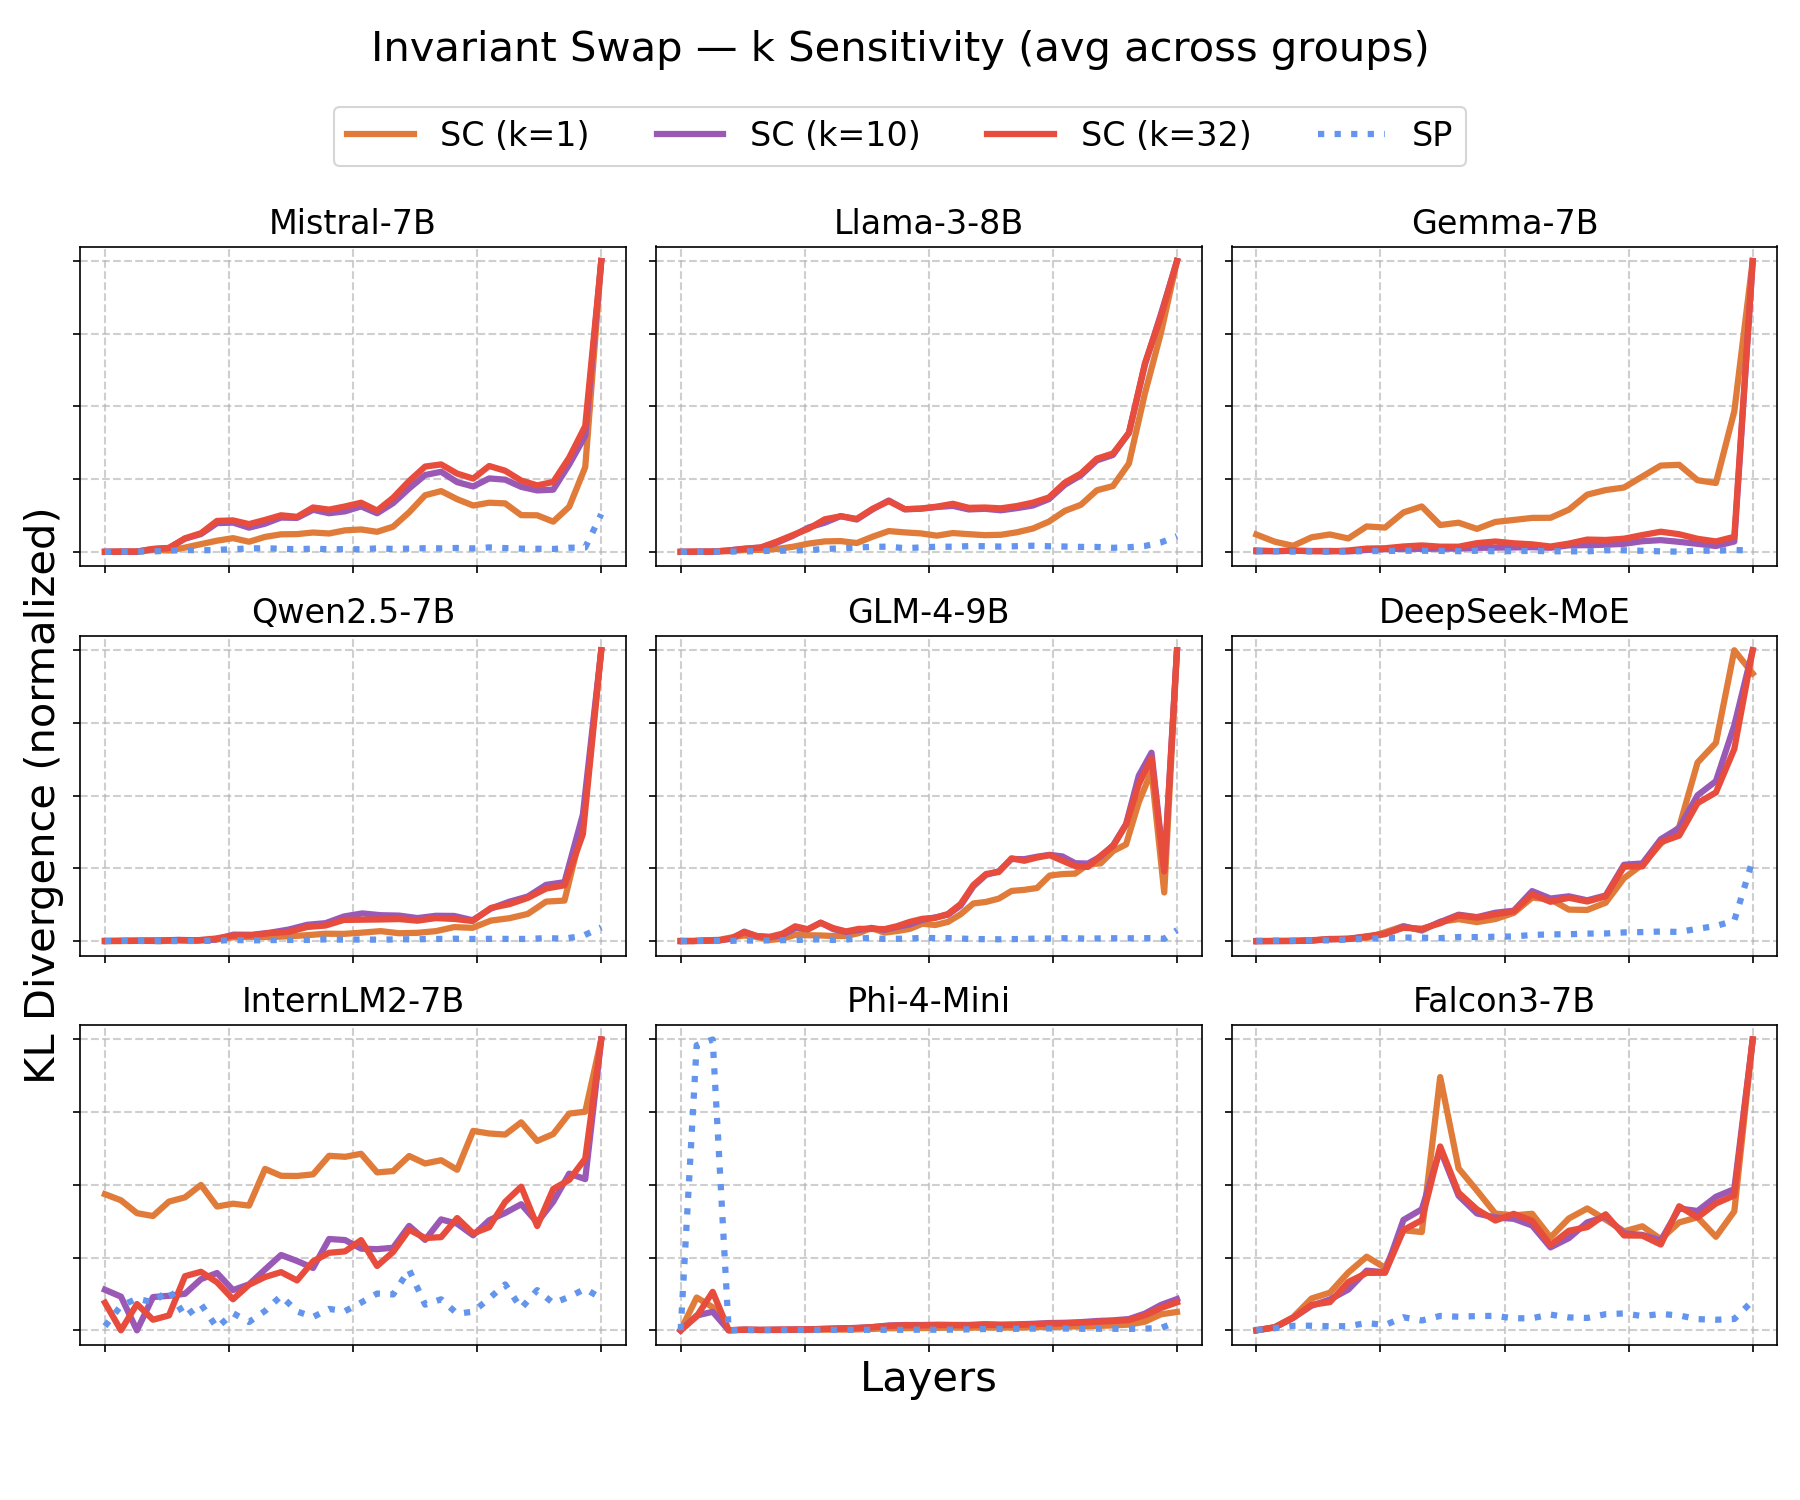
\includegraphics[width=0.8\linewidth]{figures/grid_inv_k_comparison.png}
%     \vspace{-2.0em}
%     \caption{Per-layer KL divergence for invariant component swaps across all nine models, averaged across all ten concept groups ($\alpha=1.0$). Each subplot shows three solid curves corresponding to $k \in \{1, 10, 32\}$ for SC donors, and one dotted curve for SP. SC curves increase consistently with depth while the SP curve remains near zero, confirming that the invariant subspace selectively encodes semantic content. The three SC curves closely overlap, indicating insensitivity to the choice of $k$.}
%     \label{fig:inv_k_comparison}
%     \vspace{-1.0em}
% \end{figure}

% \paragraph{Interpretation.}
% Figures~\ref{fig:inv_k_comparison} and~\ref{fig:nuis_k_comparison} report the per-layer KL divergence for invariant and nuisance component swaps respectively, averaged across all ten concept groups and all nine models. For invariant swaps, each subplot compares SC donors (semantically different) against SP donors (paraphrases) across three values of $k$. Across all architectures, the SP curves remain consistently near zero regardless of $k$, indicating that substituting the invariant component with semantically equivalent content does not perturb model predictions. In contrast, SC curves increase steadily with depth across all values of $k$, showing that injecting semantically mismatched invariant features induces a growing deviation in the output distribution.

% The divergence between SC and SP conditions becomes most pronounced in mid-to-late layers, coinciding with the layers identified as invariant zones through the generalized eigenvalue analysis in Section~\ref{sec: localize}. Early layers exhibit limited separation, consistent with their role in encoding surface-form and syntactic information prior to semantic abstraction. For nuisance swaps, both SC and SP curves increase at comparable rates with no consistent separation across layers or architectures, corroborating the diagnostic analysis in Appendix~\ref{app:nuisance_swap} and confirming that the nuisance subspace does not selectively encode semantic content.

% \begin{figure}[h]
%     \centering
%     \vspace{-1.0em}
%     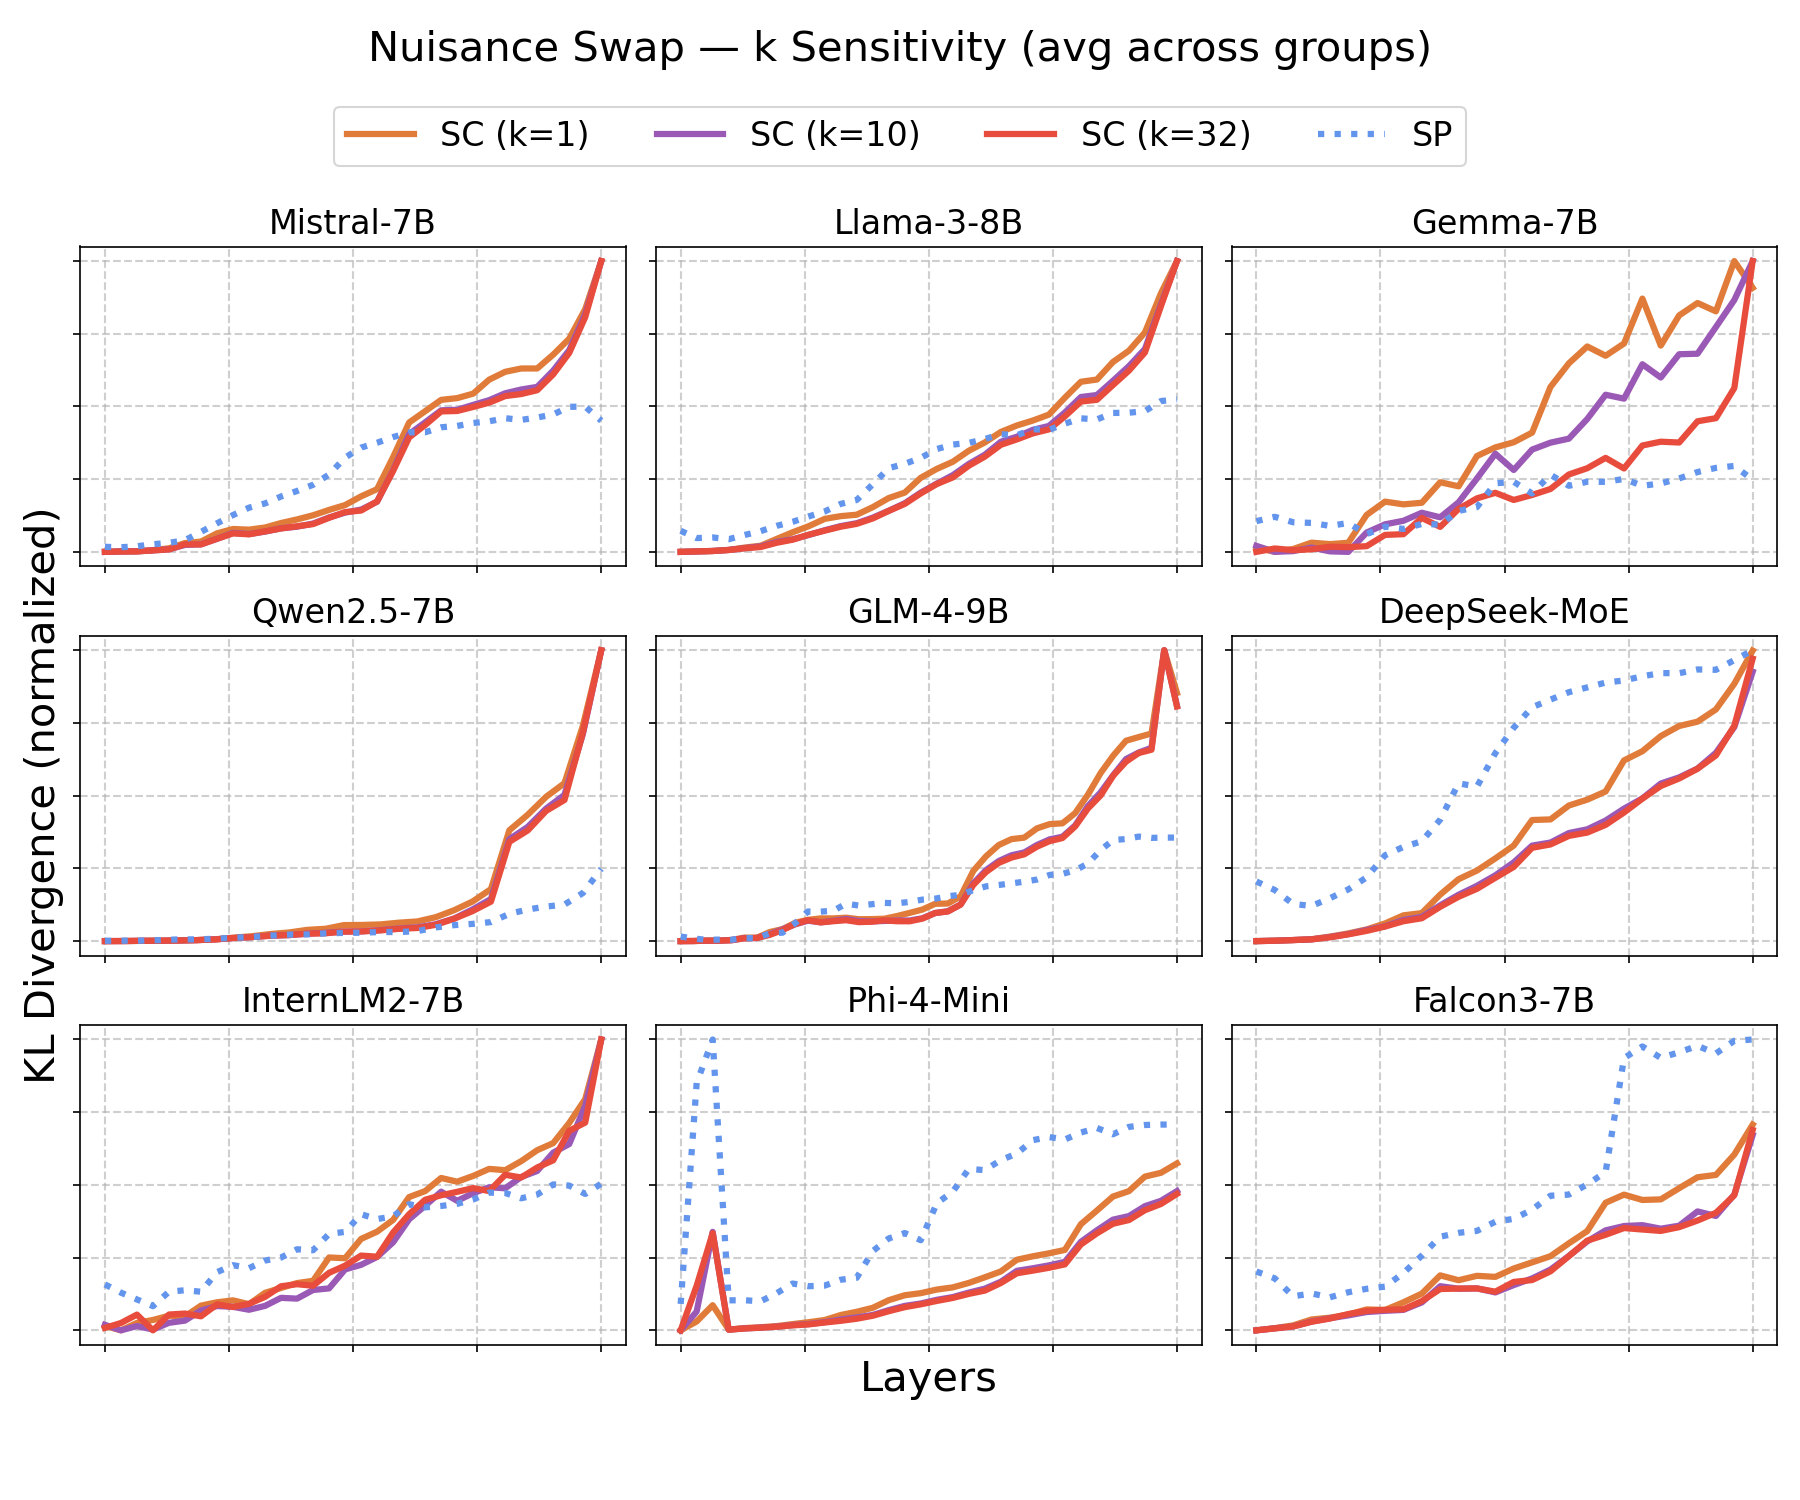
\includegraphics[width=0.8\linewidth]{figures/grid_nuis_k_comparison.png}
%     \vspace{-2.0em}
%     \caption{Per-layer KL divergence for nuisance component swaps across all nine models, averaged across all ten concept groups ($\alpha=1.0$). Each subplot shows three solid curves for SC donors at $k \in \{1, 10, 32\}$ and one dotted curve for SP donors ($k=32$). Both SC and SP curves increase at comparable rates with no consistent separation, indicating that the nuisance subspace does not selectively encode semantic content regardless of the choice of $k$.}
%     \label{fig:nuis_k_comparison}
%     \vspace{-1.0em}
% \end{figure}

% These results support two complementary conclusions that hold consistently across all models, groups, and values of $k$. First, the invariant subspace is causally relevant: interventions on this subspace directly affect model outputs in a manner that grows with layer depth. Second, the effect is semantically selective: only semantically inconsistent substitutions produce significant output shifts, confirming that the invariant component captures semantic structure rather than generic representational variation. The absence of this selectivity under nuisance swaps further validates the proposed decomposition, demonstrating that the two components play distinct and complementary roles in the representational geometry of transformer language models.

% \paragraph{Insensitivity to Subspace Dimension $k$.}
% We evaluate the sensitivity of our results to the choice of subspace dimension $k$ and observe consistent behavior for $k \in \{1, 10, 32\}$ across all experiments, as evidenced by the close overlap of the three SC curves in each subplot of Figures~\ref{fig:inv_k_comparison} and~\ref{fig:nuis_k_comparison}. This insensitivity is desirable and aligns with both the empirical structure of the data and the theoretical formulation.

% First, it suggests that invariant structure is concentrated in a low-dimensional subspace: the leading generalized eigenvectors already capture the dominant semantic directions, and increasing $k$ primarily adds weaker components with diminishing contribution. This is consistent with the eigenvalue spectrum reported in Section~\ref{sec: localize}, where a small number of directions exhibit significantly larger eigenvalues, indicating that semantic invariance is inherently low-rank.

% Second, from a theoretical perspective, the framework requires only that a subspace exists that separates semantic-preserving and semantic-changing variation; it does not depend on a precise choice of dimensionality. As long as the selected subspace captures the dominant invariant directions, downstream behavior should remain stable.

% Finally, robustness to $k$ improves practical reliability: it indicates that the identified invariant zones and downstream analyses are not sensitive to hyperparameter tuning, and that the geometric structure is a stable property of the representations rather than an artifact of a particular subspace dimension choice.


% \paragraph{Detailed Results and Interpretation.}
% Figure~\ref{fig:invariance_kl} reports the per-layer KL divergence for invariant component swaps across all models. Each subplot compares two conditions: SC donors (semantically different) and SP donors (paraphrases). Across all architectures, the SP curves remain consistently near zero, indicating that substituting invariant components with semantically equivalent content does not perturb model predictions. In contrast, SC curves increase steadily with depth, showing that injecting semantically mismatched invariant features induces a growing deviation in the output distribution.

% The divergence between SC and SP conditions becomes most pronounced in mid-to-late layers, which coincides with the layers identified as invariant zones through the generalized eigenvalue analysis. Early layers exhibit limited separation, consistent with their role in encoding surface-form and syntactic information prior to semantic abstraction.

% These results support two complementary conclusions. First, the invariant subspace is causally relevant: interventions on this subspace directly affect model outputs. Second, the effect is semantically selective: only semantically inconsistent substitutions produce significant changes, confirming that the invariant component captures semantic structure rather than generic variation. Additional results across all concept groups are provided in Appendix~\ref{app:all_groups}.



In practice, $S_{\mathrm{sp}}$ is low rank because the number of semantic-preserving perturbations is much smaller than the hidden dimension. We therefore solve a regularized generalized eigenvalue problem,
\[
S_{\mathrm{sc}} v = \lambda (S_{\mathrm{sp}} + \epsilon I)v,
\]
where $\epsilon > 0$ ensures numerical stability. Let $V_{\ell}^{\mathrm{inv}} = [v_1, \ldots, v_k]$ denote the top-$k$ generalized eigenvectors with the largest eigenvalues at layer $\ell$. 

Since generalized eigenvectors are orthogonal with respect to the $(S_{\mathrm{sp}} + \epsilon I)$-inner product but not necessarily under the Euclidean inner product, we compute an orthonormal basis
\[
U_\ell^{\mathrm{inv}} = \mathrm{orth}(V_\ell^{\mathrm{inv}})
\]
via QR decomposition. This ensures that $U_\ell^{\mathrm{inv}} U_\ell^{\mathrm{inv}\top}$ defines a valid Euclidean projection operator.

The invariant representation at layer $\ell$ is then obtained by projection,
\begin{equation}
z_{\mathrm{inv}}
=
U_\ell^{\mathrm{inv}}
U_\ell^{\mathrm{inv}\top} z .
\label{eq: decompose_z_inv}
\end{equation}
This projection suppresses nuisance-sensitive components while preserving directions that remain stable under paraphrasing yet discriminate across meanings. 

The complementary nuisance component is given by
\[
z_{\mathrm{nuis}}
=
\left(
I-
U_\ell^{\mathrm{inv}}
U_\ell^{\mathrm{inv}\top}
\right) z.
\]


\aat{Table~\ref{tab:causal_intervention_analysis} presents causal intervention results obtained by patching invariant and nuisance components across multiple language models. For each semantic group, we first discover invariant directions by solving the generalized eigenvalue problem and selecting the top-$k$ eigenvectors associated with the largest generalized eigenvalues. The top-4 layers are then selected according to the largest leading eigenvalue $\lambda$, corresponding to layers exhibiting the strongest semantic–nuisance separation. At each selected layer, token-level hidden states are decomposed into invariant and nuisance components through orthogonal projection onto the discovered subspaces. Interventions are then applied directly to hidden states before propagating the modified activations through the remaining frozen transformer layers.

We evaluate both semantic-preserving and semantic-changing interventions by independently replacing either the invariant or nuisance component while keeping the complementary component fixed. Model behavior before and after intervention is compared using KL divergence and logit-space mean squared error (MSE). If the discovered decomposition is meaningful, interventions within the nuisance subspace should induce relatively small output changes, whereas interventions within the invariant subspace should produce substantially larger semantic shifts, particularly when donor representations originate from semantically different groups. Across models, the observed trends consistently support this hypothesis: nuisance interventions generally preserve model outputs, while invariant interventions produce significantly larger deviations in the predicted token distributions. These results provide causal evidence that the discovered invariant directions encode semantic structure, whereas nuisance directions primarily capture semantic-preserving variability.}


\section{Ablation Study: More Results on Causal Validation via Representation Intervention}
\label{append: between_group}

We extend the representation-level intervention framework in Section 4.4 to a more stringent setting, where donor representations are drawn from \emph{different semantic groups}. This experiment evaluates whether the invariant subspace encodes consistent semantic structure beyond within-group paraphrastic variation.

\vspace{-0.8em}
\paragraph{Experimental Setup.}
The intervention follows the same formulation as Section~\ref{sec:ab_mainpaper}, operating on token-level hidden states. For an anchor input $x^{(a)}$ from semantic group $g$ and a donor input $x^{(d)}$ from a different group $h \neq g$, we construct intervened representations by modifying either the invariant or nuisance component while keeping the complementary component fixed.

For invariant intervention, we replace the invariant component:
\(
h^{\text{int}} = h^{(a)} + \alpha \big(h^{(d)}_{\text{inv}} - h^{(a)}_{\text{inv}}\big),
\)
while for nuisance intervention, we replace the nuisance component:
\(
h^{\text{int}} = h^{(a)} + \big(h^{(d)}_{\text{nuis}} - h^{(a)}_{\text{nuis}}\big).
\)

The modified representation is injected at layer $\ell$ and propagated forward to produce output logits.

Unlike within-group interventions, between-group interventions introduce a group-wise semantic mismatch between anchor and donor. We evaluate the effect of these interventions using Mean Squared Error (MSE) between output representations and KL divergence between next-token distributions.



\paragraph{Results.}
The results are summarized in Tables~\ref{tab:between_group_nuis} and~\ref{tab:between_group_inv}. A clear asymmetry emerges between nuisance and invariant interventions across all models and semantic groups.

First, nuisance-component swaps (Table~\ref{tab:between_group_nuis}) produce consistently low MSE and KL divergence. Despite the donor being drawn from a different semantic group, replacing the nuisance component induces only limited changes in the model output. This indicates that the nuisance subspace does not carry primary semantic information and that cross-group variation in this subspace has relatively weak causal impact.

In contrast, invariant-component swaps (Table~\ref{tab:between_group_inv}) produce large and consistent deviations, reflected in high normalized MSE and KL values across all models. Replacing the invariant component with that of a semantically different input induces a strong and systematic shift in model behavior, confirming that this subspace encodes semantic identity at a global level.

Importantly, this pattern is highly consistent across model families and semantic groups. Together with within-group results, these findings provide complementary causal evidence: perturbations in the invariant subspace induce semantic changes, whereas perturbations in the nuisance subspace have comparatively limited effect.

\paragraph{Discussion.}
Compared to within-group interventions, the between-group setting removes residual lexical and structural similarity, isolating the role of representation geometry. The observed asymmetry between invariant and nuisance interventions therefore reflects intrinsic properties of the learned subspaces rather than dataset artifacts.

The results support a clear causal interpretation of the decomposition: the invariant subspace encodes semantically meaningful directions that govern model behavior, while the nuisance subspace captures variation that is largely orthogonal to semantic identity. Although nuisance components may still influence outputs, their effect is not semantically structured and remains substantially weaker than that of invariant components.